\documentclass[a4paper, landscape]{article}

\usepackage[DIV=18]{typearea}
\usepackage{microtype}
\usepackage{float}
\usepackage{mathtools, amssymb}
\usepackage{bbm}
\usepackage{parskip}
\usepackage[colorlinks=true]{hyperref}

\hypersetup{linktoc=all}

\setcounter{MaxMatrixCols}{20}

\title{2}
\date{}

\begin{document}
\maketitle
\section{Background}
The image intensity is given in the below form
\begin{equation}{\label{eq:bcip}}
		v(x,y)= \sum_{i=0}^{3}\sum_{j=0}^{3} a_{ij}x^i y^j
\end{equation}
Let the 16 nearest points be $(x_i, y_i)$ where $i\in\{1,2,\dots,16\}$ and their corresponding intensities are given by $v(x_i, y_i)$.
Currently all $a_{ij}$ are unknown, but we can solve them by combining \ref{eq:bcip} for all these 16 points using matrix representation as shown below 
\begin{equation}
    \underbrace{
    \begin{bmatrix}
        v(x_1, y_1)\\
        v(x_2, y_2)\\
        v(x_3, y_3)\\
        v(x_4, y_4)\\
        v(x_5, y_5)\\
        v(x_6, y_6)\\
        v(x_7, y_7)\\
        v(x_8, y_8)\\
        v(x_9, y_9)\\
        v(x_{10}, y_{10})\\
        v(x_{11}, y_{11})\\
        v(x_{12}, y_{12})\\
        v(x_{13}, y_{13})\\
        v(x_{14}, y_{14})\\
        v(x_{15}, y_{15})\\
        v(x_{16}, y_{16})\\
    \end{bmatrix}
    }_{v}=
    \underbrace{
    \begin{bmatrix}
        1 & y_1 & y_1^2 & y_1^3 & x_1 & x_1y_1 & x_1y_1^2 & x_1y_1^3 & x_1^2 & x_1^2y_1 & x_1^2y_1^2 & x_1^2y_1^3 & x_1^3 & x_1^3y_1 & x_1^3y_1^2 & x_1^3y_1^3\\
        1 & y_2 & y_2^2 & y_2^3 & x_2 & x_2y_2 & x_2y_2^2 & x_2y_2^3 & x_2^2 & x_2^2y_2 & x_2^2y_2^2 & x_2^2y_2^3 & x_2^3 & x_2^3y_2 & x_2^3y_2^2 & x_2^3y_2^3\\
        1 & y_3 & y_3^2 & y_3^3 & x_3 & x_3y_3 & x_3y_3^2 & x_3y_3^3 & x_3^2 & x_3^2y_3 & x_3^2y_3^2 & x_3^2y_3^3 & x_3^3 & x_3^3y_3 & x_3^3y_3^2 & x_3^3y_3^3\\
        1 & y_4 & y_4^2 & y_4^3 & x_4 & x_4y_4 & x_4y_4^2 & x_4y_4^3 & x_4^2 & x_4^2y_4 & x_4^2y_4^2 & x_4^2y_4^3 & x_4^3 & x_4^3y_4 & x_4^3y_4^2 & x_4^3y_4^3\\
        1 & y_5 & y_5^2 & y_5^3 & x_5 & x_5y_5 & x_5y_5^2 & x_5y_5^3 & x_5^2 & x_5^2y_5 & x_5^2y_5^2 & x_5^2y_5^3 & x_5^3 & x_5^3y_5 & x_5^3y_5^2 & x_5^3y_5^3\\
        1 & y_6 & y_6^2 & y_6^3 & x_6 & x_6y_6 & x_6y_6^2 & x_6y_6^3 & x_6^2 & x_6^2y_6 & x_6^2y_6^2 & x_6^2y_6^3 & x_6^3 & x_6^3y_6 & x_6^3y_6^2 & x_6^3y_6^3\\
        1 & y_7 & y_7^2 & y_7^3 & x_7 & x_7y_7 & x_7y_7^2 & x_7y_7^3 & x_7^2 & x_7^2y_7 & x_7^2y_7^2 & x_7^2y_7^3 & x_7^3 & x_7^3y_7 & x_7^3y_7^2 & x_7^3y_7^3\\
        1 & y_8 & y_8^2 & y_8^3 & x_8 & x_8y_8 & x_8y_8^2 & x_8y_8^3 & x_8^2 & x_8^2y_8 & x_8^2y_8^2 & x_8^2y_8^3 & x_8^3 & x_8^3y_8 & x_8^3y_8^2 & x_8^3y_8^3\\
        1 & y_9 & y_9^2 & y_9^3 & x_9 & x_9y_9 & x_9y_9^2 & x_9y_9^3 & x_9^2 & x_9^2y_9 & x_9^2y_9^2 & x_9^2y_9^3 & x_9^3 & x_9^3y_9 & x_9^3y_9^2 & x_9^3y_9^3\\
        1 & y_{10} & y_{10}^2 & y_{10}^3 & x_{10} & x_{10}y_{10} & x_{10}y_{10}^2 & x_{10}y_{10}^3 & x_{10}^2 & x_{10}^2y_{10} & x_{10}^2y_{10}^2 & x_{10}^2y_{10}^3 & x_{10}^3 & x_{10}^3y_{10} & x_{10}^3y_{10}^2 & x_{10}^3y_{10}^3\\
        1 & y_{11} & y_{11}^2 & y_{11}^3 & x_{11} & x_{11}y_{11} & x_{11}y_{11}^2 & x_{11}y_{11}^3 & x_{11}^2 & x_{11}^2y_{11} & x_{11}^2y_{11}^2 & x_{11}^2y_{11}^3 & x_{11}^3 & x_{11}^3y_{11} & x_{11}^3y_{11}^2 & x_{11}^3y_{11}^3\\
        1 & y_{12} & y_{12}^2 & y_{12}^3 & x_{12} & x_{12}y_{12} & x_{12}y_{12}^2 & x_{12}y_{12}^3 & x_{12}^2 & x_{12}^2y_{12} & x_{12}^2y_{12}^2 & x_{12}^2y_{12}^3 & x_{12}^3 & x_{12}^3y_{12} & x_{12}^3y_{12}^2 & x_{12}^3y_{12}^3\\
        1 & y_{13} & y_{13}^2 & y_{13}^3 & x_{13} & x_{13}y_{13} & x_{13}y_{13}^2 & x_{13}y_{13}^3 & x_{13}^2 & x_{13}^2y_{13} & x_{13}^2y_{13}^2 & x_{13}^2y_{13}^3 & x_{13}^3 & x_{13}^3y_{13} & x_{13}^3y_{13}^2 & x_{13}^3y_{13}^3\\
        1 & y_{14} & y_{14}^2 & y_{14}^3 & x_{14} & x_{14}y_{14} & x_{14}y_{14}^2 & x_{14}y_{14}^3 & x_{14}^2 & x_{14}^2y_{14} & x_{14}^2y_{14}^2 & x_{14}^2y_{14}^3 & x_{14}^3 & x_{14}^3y_{14} & x_{14}^3y_{14}^2 & x_{14}^3y_{14}^3\\
        1 & y_{15} & y_{15}^2 & y_{15}^3 & x_{15} & x_{15}y_{15} & x_{15}y_{15}^2 & x_{15}y_{15}^3 & x_{15}^2 & x_{15}^2y_{15} & x_{15}^2y_{15}^2 & x_{15}^2y_{15}^3 & x_{15}^3 & x_{15}^3y_{15} & x_{15}^3y_{15}^2 & x_{15}^3y_{15}^3\\
        1 & y_{16} & y_{16}^2 & y_{16}^3 & x_{16} & x_{16}y_{16} & x_{16}y_{16}^2 & x_{16}y_{16}^3 & x_{16}^2 & x_{16}^2y_{16} & x_{16}^2y_{16}^2 & x_{16}^2y_{16}^3 & x_{16}^3 & x_{16}^3y_{16} & x_{16}^3y_{16}^2 & x_{16}^3y_{16}^3\\
    \end{bmatrix}
    }_{M}
    \underbrace{
    \begin{bmatrix}
    a_{00}\\
    a_{01}\\
    a_{02}\\
    a_{03}\\
    a_{10}\\
    a_{11}\\
    a_{12}\\
    a_{13}\\
    a_{20}\\
    a_{21}\\
    a_{22}\\
    a_{23}\\
    a_{30}\\
    a_{31}\\
    a_{32}\\
    a_{33}\\
    \end{bmatrix}
    }_{a}\label{eq:g}
\end{equation}
Now, the analysis of invertibility of this matrix seems non-trivial. As mentioned in SIAM by \href{https://evoq-n.org/Portals/0/Publications/SIURO/Vol1_Issue1/A_Simple_Expression_for_Multivariate.pdf}{Kamron}, any arbitrary multivariate polynomial of $m$ variables and degree $n$ may need upto $\binom{n+m}{n}$ distinct points and their evaluations to uniquely interpolate the coefficients. Since $\binom{6+2}{2}=28$ and $28>16$, this theorem will not help us and we will need to utilise some special structure of this bicubic expression to prove that this matrix $M$ is invertible for distinct points if that is the case. Anyway, if $M$ is invertible then the coefficients can be calculated as follow
\begin{equation}
    a = M^{-1} v
\end{equation}
\section{Assumption}
Since, there are 16 variables in \ref{eq:g}, {atleast 16 equations} are needed according to linear algebra. Hence, \textbf{atleast 16 points} are needed to get these coefficients.

Now, we will show that it can be done in 16 points with a suitable assumption.

For this, we have to assume that the \textbf{16 nearest neighbors} as mentioned in the question form a grid. Though this sounds trivial, the 16 nearest neighbors don't actually form a grid in our usual notion of euclidean distance. By symmetry, the candidate $4\times4$ grid that contains the 16 nearest neighbors must have the given point (shown in red) inside or on the $1\times1$ grid at the center. Figure \ref{fig:nearest} shows this as if a point is not in the center $1\times1$ part of the grid (unshaded), there exists a grid (shaded) that include some points that are `nearer' to the given point but not in the grid (unshaded). 

Figure \ref{fig:nearest} also shows the other side of the problem, that even the best grid does not contain all the 16 nearest neighbours. As, even if we pick this suitable grid (shaded) following the above rule there are still some omitted lattice points in unshaded region that are actually `closer' than some lattice points in the shaded region.

But this problem can be easily solved by changing our distance metric to $\max-$norm. Now, the candidate grid we discussed always contains the 16 nearest neighbours as any lattice point in the grid is at at most 2 units from the given point and any lattice point on outside is at least 2 units from the given point. The equality occurring when the given point is on the boundary of the $1\times1$ center grid.
\begin{figure}[H]
    \centering
    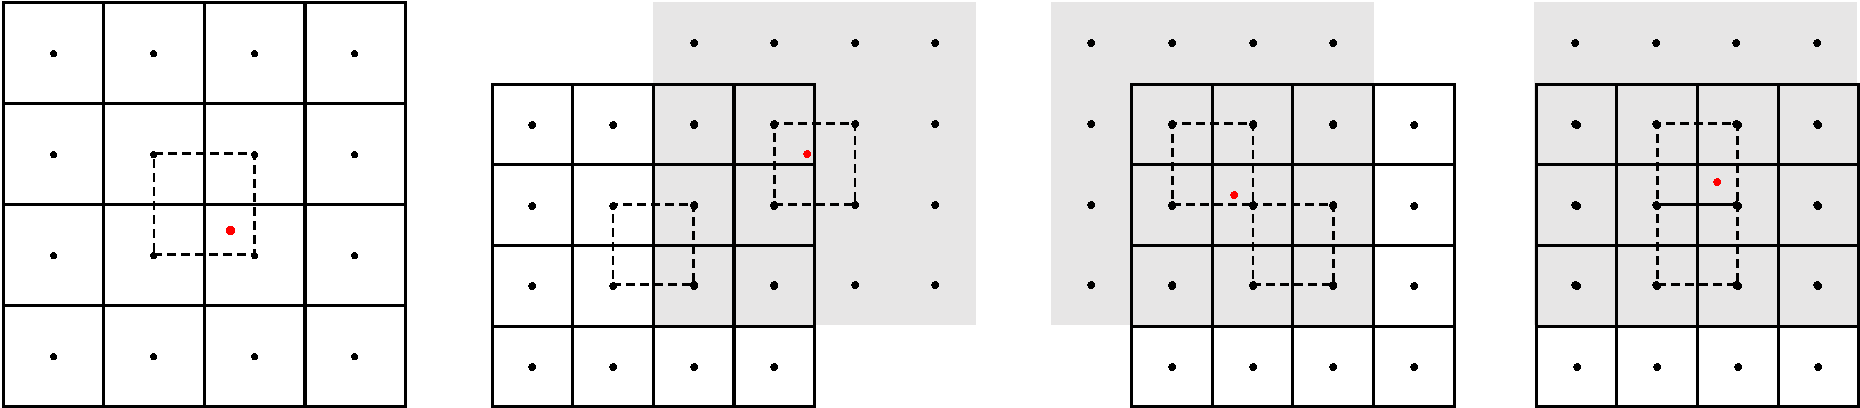
\includegraphics[width=\linewidth]{nearest_point.pdf}
    \caption{Leftmost figure denotes the rule to select 16 nearest points to the given point, other figures denote the 16 nearest points around the given point not in the center grid.}
    \label{fig:nearest}
\end{figure}
\section{Solution}
Now, we can the points as $(p,q)$ where $p\in\{x,x+1,x+2,x+3\}$ and $q\in\{y,y+1,y+2,y+3\}$. With this formulation, the given point $(x_0,y_0)$ is such that $x+1\leq x_0\leq x+2$ and $y+1\leq y_0\leq y+2$. Now, \ref{eq:bcip} can also be written as
\begin{equation}
    v(x,y)=\begin{bmatrix}
        1 & x & x^2 & x^3
    \end{bmatrix}
    \begin{bmatrix}
        a_{00} & a_{01} & a_{02} & a_{03}\\
        a_{10} & a_{11} & a_{12} & a_{13}\\
        a_{20} & a_{21} & a_{22} & a_{23}\\
        a_{30} & a_{31} & a_{32} & a_{33}\\
    \end{bmatrix}
    \begin{bmatrix}
        1 \\ y \\y^2 \\ y^3
    \end{bmatrix}
\end{equation}
Hence, these can be easily combined for the grid coordinates as follows:
\begin{equation}
    \underbrace{
    \begin{bmatrix}
        v(x,y) & v(x,y+1) & v(x,y+2) & v(x,y+3)\\
        v(x+1,y) & v(x+1,y+1) & v(x+1,y+2) & v(x+1,y+3)\\
        v(x+2,y) & v(x+2,y+1) & v(x+2,y+2) & v(x+2,y+3)\\
        v(x+3,y) & v(x+3,y+1) & v(x+3,y+2) & v(x+3,y+3)\\
    \end{bmatrix}
    }_{V}
    =
    \underbrace{
    \begin{bmatrix}
        1 & x & x^2 & x^3\\
        1 & x+1 & (x+1)^2 & (x+1)^3\\
        1 & x+2 & (x+2)^2 & (x+2)^3\\
        1 & x+3 & (x+3)^2 & (x+3)^3\\
    \end{bmatrix}
    }_{V_x}
    \underbrace{
    \begin{bmatrix}
        a_{00} & a_{01} & a_{02} & a_{03}\\
        a_{10} & a_{11} & a_{12} & a_{13}\\
        a_{20} & a_{21} & a_{22} & a_{23}\\
        a_{30} & a_{31} & a_{32} & a_{33}\\
    \end{bmatrix}
     }_{A}
    \underbrace{
    \begin{bmatrix}
        1 & 1 & 1 & 1 \\ y & y+1 & y+2 & y+3 \\y^2 & (y+1)^2 & (y+2)^2 & (y+3)^2  \\ y^3 & (y+1)^3 & (y+2)^3 & (y+3)^3
    \end{bmatrix}
     }_{V_y^T}
\end{equation}
where $V_x, V_y$ are the Vandermonde matrices which are invertible for distinct values and as the inverse of a square matrix is unique the determined coefficients are unique. 
\begin{equation}
    A = V_x^{-1} V (V_y^{T})^{-1}
\end{equation}
We initially showed that atleast 16 neighbours are necessary and now we have shown that they are sufficient to calculate the coefficients uniquely.
%$(x,y), (x,y+1), (x,y+2), (x, y+3), (x+1,y), (x+1,y+1), (x+1,y+2), (x+1, y+3), (x+2,y), (x+2,y+1), (x+2,y+2), (x+2, y+3), (x+3,y), (x+3,y+1), (x+3,y+2), (x+3, y+3)$
% Let us consider a neighbourhood containing 16 pixels arranged in a $4\times 4$ grid. Now, for these pixels their $x-$coordinate $\in\{p,p+1,p+2,p+3\}$ and $y-$coordinate $\in\{q,q+1,q+2,q+3\}$
% Let us consider that the given point in somewhere 
\end{document}
